\chapter{Vagueness ($\catZ$)}
\label{ch:vagueness}
\begin{flushright}
\emph{An approximate answer to the right question is better than\\
a precise answer to the wrong question.} --- John Tukey (rephrased)
\end{flushright}
\minitoc

NOTE:  this section will be re-formulated soon.  In the new version I only make 2 assumptions:

1. There are some quantities known as "degrees" and they are normalized to [0,1].

2. There exist relations amongst these quantities captured by \textbf{statistical models}.

I think the new formulation will be fairly unblemishable and uncontroversial, as opposed to earlier forms of fuzzy logic which many people are skeptical of.  But the new version also falls out of the classification as logic and is more of a fuzzy-probabilistic calculus.
\\

\footnotesize
I use $\catZ$ instead of $\mathcal{F}$ to denote fuzziness partly in recognition of Lotfi Zadeh's contributions, and also because $F$ and $f$ are often used for the CDF and PDF in probability theory, which may cause confusion when probabilities and fuzziness are used together.

A note on the examples used in this book:  some of them are politically incorrect or somewhat embarrassing.  I prefer examples that are simple, realistic, and relevant to human emotions because they help us think more clearly (cf the Wason selection task).  Usually I just choose the most obvious examples that come to mind.
\normalsize

\section{Vague phenomena}

There seems to be 3 types of concepts (= predicates).

The first type is \textbf{discrete} in nature, for example\footnote{I will later argue that even these concepts are not completely binary.}:\\
\hspace*{1cm} sex of a person $\in$ \{ male, female, hermaphrodite, trans-sexual \}\\
\hspace*{1cm} marital status $\in$ \{ single, engaged, married, divorced \}

The second type represents \textbf{numerical} measures, for example:\\
\hspace*{1cm} height \hspace*{1cm} weight \hspace*{1cm} age

The third type is not strictly numerical, but is often associated with ``\textbf{gradedness}'':\\
\hspace*{0.8cm} \begin{tabular}{l l}
beautiful    & ugly\\
intelligent  & dumb\\
simple       & complex\\
interesting  & boring\\
good         & bad\\
easy         & difficult\\
friendly     & hostile\\
clear        & unclear
\end{tabular}

There is no doubt that these predicates can be modified with degrees like ``very'' or ``slightly''.  But we do not know of any exact measures of their degrees.  For example, IQ has been proposed as an inexact measure of intelligence.  Most people would agree that there is some general consensus as to what is intelligent.  Such concepts exhibit \textit{vague phenomena}, which are characterized by:\\
\hspace*{1cm} 1. borderline cases\\
\hspace*{1cm} 2. lack of sharp boundaries\\
\hspace*{1cm} 3. susceptible to sorites paradox\footnote{A solution to the sorites paradox is given in \citep*{Bergmann2008} p268-282, using fuzzy logic and the notion of \textit{decaying validity}.}\\
\hspace*{1cm} 4. open-texture (ie, if $x$ is a borderline case, one can assert either $Q(x)$ or $\neg Q(x)$ in different contexts)

In philosophical logic, there are a number of theories of vagueness (see eg, \citep*{Graff2002}, \citep*{Keefe2000}, \citep*{Shapiro2006}).  $\catZ$ logic is a kind of Degree Theory (\citep*{Edgington1992}, \citep*{Sainsbury1986}), that uses numerical truth values to represent vagueness.  There are other non-numerical theories such as Epistemicism (\citep*{Campbell1974}, \citep*{Williamson1994}), and Supervaluation (\citep*{Fine1975}, \citep*{Keefe2000}).

\section{Why vagueness is needed for AGI}
\label{sec:whyZ}

One of the critical capabilities of AGI is (self-)programming.  Also, it is imperative to be able to instruct an AGI to write programs according to \textit{natural language} specifications and with robust common-sense background knowledge.  common-sense reasoning and natural language understanding depend on the use of vague concepts.\footnote{Vague concepts are not required for formal reasoning tasks such as formal mathematics and programming according to formal specifications.}  Look at any (technical or non-technical) natural-language text, and one finds that (explicit or implicit) vague concepts are ubiquitous.  It seems to be occur even more frequently than the (explicit or implicit) use of probabilities.

\textbf{Ubiquity of vagueness in common-sense reasoning.}  Some examples are:\\
\textbullet \, Time: \textit{Mother died \underline{a few days ago}}\\
\textbullet \, Space: \textit{One bird flew \underline{over the cuckoo's nest}} \hspace*{0.5cm} (lacking exact boundaries)\\
\textbullet \, Physics of liquids: \textit{A liquid in bulk and at rest has a horizontal surface}\\ (Is soup a liquid? ``In bulk'' is a fuzzy concept. Is the sea at rest? Surface tension can cause surface to curve)\\
\textbullet \, Physics of solids: \textit{A solid object cannot go from inside to outside a closed box}\\  (``Solid object'' is a fuzzy concept (eg a block of ice, a cat, a bomb). A card box may have small holes. The lid may be slightly ajar.)
%\textbullet \, Minds: 
%\textbullet 
%\textbullet 

\section{Why \textit{numerical} vagueness?}

The controversy is whether vagueness should be managed \textbf{quantitatively} (such as $\catZ$) or \textbf{qualitatively}.

One objection is that fuzzy logic can sometimes lead to unsound conclusions.  This problem is discussed in \S\ref{sec:exceptions} on nonmonotonic reasoning.

Having numerical vagueness allows us to:\\
1. Represent quantitative rules.  For example:\\
\hspace*{1cm} \begin{tabular}{l l l}
smart & $\leftarrow$ eloquent    & (the more articulate the smarter)\\
      & $\leftarrow$ humorous    & (the more humorous the smarter)\\
      & $\leftarrow$ insightful  & (the more insightful the smarter)\\
      & $\leftarrow$ creative    & (the more creative the smarter)\\
      & $\leftarrow$ etc...      &
\end{tabular}\\
2. Add up graded factors.  For example:\\
\hspace*{1cm} ``John is eloquent, humorous, insightful and creative'' $\rightarrow$ 0.9 smart\\
\hspace*{1cm} ``John is humorous and nothing else'' $\rightarrow$ 0.6 smart\\
3. Accrue contributing factors of a concept over a long period of time:\\
\hspace*{1cm} ``From my long experience with John, he is 0.9 smart''.

On the other hand, if we do not use numerical vagueness, we face these problems:\\
1. Failure to recognize ``partial'' concepts.  For example:\\
\hspace*{1cm} ``John is 0.7 smart'', or\\
\hspace*{1cm} ``tomato is 0.7 a fruit''\\
2. Conversely, failure to ignore ``very weak'' partial concepts.\\
3. Each statement must be attached with many qualifications, and they keep accumulating. Each rule would have to recognize a large ``exception set''.

The solution I adopt is to use both qualitative and quantitative information, by representing facts \textit{redundantly} (\S\ref{sec:exceptions}).  For example:\\
\hspace*{1cm} ``John is smart'', $z = 0.7$ (quantitative)\\
\hspace*{1cm} ``But he is only penny wise'' (qualitative)

Lastly, what if we don't need the precision of numerical vagueness in some situations?  For example:\\
\hspace*{1cm} ``Is John really that smart?'' ``Not quite.'' (we don't know the exact degree of smartness)\\
or\\
\hspace*{1cm} ``John is slightly smarter than Peter.'' (but we don't know the exact difference)\\
In my theory, these cases can be handled by combining $\catP$ and $\catZ$.

%One suggestion is that we can always use \textit{qualitative} binary statements in place of quantitative ones:\\
%\hspace*{1cm} ``John is fairly intelligent''\\
%\hspace*{1cm} \texttt{intelligent$_1$(john), fairly(intelligent$_1$)}\\
%\hspace*{1cm} ``John is intelligent but only in small matters''\\
%\hspace*{1cm} \texttt{intelligent$_1$(john), qualifies(intelligent$_1$, "only in small matters")}\\
%For the second example, we may say that a person who is intelligent only in small matters is not very intelligent, and thus assign, \textit{eg} Z = 0.6, but some qualitative information would be lost using this numerical representation.

%\begin{tabbing}The following example suggests that at least some \textbf{ordinal} relations may be necessary:\\
%\hspace*{1cm} (A) recently there's been a lot of thefts\hspace*{2cm} \=`that's bad'\\
%\hspace*{1cm} (B) recently there's been a lot of rapes \>`that's very bad'\\
%\hspace*{1cm} (C) recently there's been a lot of murders \>`that's extremely bad' ''
%\end{tabbing}
%which seems to suggest that the severity of crimes has this order:\\
%\hspace*{1cm} theft $<$ rape $<$ murder\\
%but this general ordering can have exceptions depending on circumstances.

%This example shows that sometimes \textbf{quantitative} representations may be necessary:\\
%\hspace*{1cm} ``During the financial crisis,\\
%\hspace*{1cm} (A) many people committed suicide;\\
%\hspace*{1cm} (B) children were sold as prostitutes;\\
%\hspace*{1cm} (C) decades of savings were destroyed''
%So one may react with the feeling ``that's very bad''.  But how was ``\underline{very} bad'' inferred?  Assuming we have a KB that let us infer that:\\
%\hspace*{1cm} A $\rightarrow$ bad\\
%\hspace*{1cm} B $\rightarrow$ bad\\
%\hspace*{1cm} C $\rightarrow$ bad\\
%how can we deduce ``very bad''?  We have 3 heterogeneous contributing factors.  One plausible solution is to assign degrees of badness to each of A, B, and C, and then add them up.

%Note that this example should be a simple reasoning task involving only a few inference steps.

%If the 3 contributing factors \textit{add up} to yield ``very bad'' (even approximately), the individual factors must be \textit{numerical}.  Or, maybe it is a simple counting of contributing factors?  3 bad things?  Not very satisfactory --- the things can have varying degrees.

%``I'm even more sure I don't want to be prostitute, after seeing the bad conditions''.  This is binary.

%But sometimes a rule for a predicate has many antecedents and only some of them are satisfied.  In the binary approach we may qualify them as exceptions.  But there are often many factors that may contribute to a predicate such as $smart$ or $charismatic$.  If you have known John for 10 years there may have been many incidences where he was smart/dumb or charismatic/dull.  In that case we may want to ``add up'' all those contributions.  In other words, it may be desirable to use a single number to summarize a large number of contributions, as long as the contributions are not exceptional.

%Suppose the AGI wants to erect these hypotheses:\\
%\hspace*{1cm} kind $\leftarrow$ attractive\\
%\hspace*{1cm} humorous $\leftarrow$ charismatic

%What if Z is not needed.  All we need is to convert results to binary, qualified form?

%Also, might it be necessary to use numerical Z even for single inference steps?\\
%For example:\\
%sluttish $\rightarrow$ not good wife (Z to Z)\\
%criminal $\rightarrow$ should be punished (Z to Z)\\
%obscene $\rightarrow$ should avoid speaking (Z to Z)\\
%attractive $\rightarrow$ I like (Z to Z)

%During pattern recognition it is often necessary to recognize an entity \textit{partially}, for example, the picture below may be a ``0.7 face''.  It seems that fuzziness is needed at a very fundamental level.
%\begin{figure}[H]
%\centering
%\input{CrossEyesFace}
%\caption{a fuzzy face}
%\end{figure}

\section{Semantics of Z}

There is some confusion about the interpretation of fuzziness, which I will try to clarify here.  I am influenced by Pei Wang's ideas \citep*{Wang2006}.

$\catZ$ is a measure of \textit{degree} or \textit{gradedness}.  Standard fuzzy theory employs the ``membership function'' to represent \textit{the degree to which an element belongs to a class}, but there is no consensus as to how the membership functions are defined.  Let's think of ``the degree to which a person is smart'', is it really arbitrary?

While there are no exact procedures to measure vague concepts (eg smartness), it is mandatory that a common-sense machine should possess some ways of assessing them, just like the human brain does.  In my AGI this is achieved by having a comprehensive knowledgebase of rules (acquired via machine learning) that compute numerical degrees of concepts.  Such rules are mini-algorithms (or ``\textbf{micro-theories}''\footnote{The term is used informally, not referring to Guha's notion of micro-theories in Cyc.}) that are \textbf{emergent properties} of intelligent learning systems.  They establish a \textit{distributed and approximate consensus} of how to measure vague concepts.

From another perspective:  PCA (principal component analysis) can calculate the component of a dataset that represents its greatest variance.  For example, PCA may identify the male-female axis of a set of movie-goers, or the liberal-conservative axis of a group of politicians.  When we map this axis to [0,1], we can get a fuzzy value of the concept male/female or liberal/conservative.  This may answer the question ``where do fuzzy numbers come from?'' \footnote{Abram Demski suggested this to me in discussion.}

If we regard $\catZ$ as a measure of degrees, $\catZ$ theory is mathematically as rigorous as probability theory.  $\catZ$ is a measure of degrees just as the height $H$ is a measure of how tall an object is.  Also, the $\catZ$-value can be inexact just as $H$ can be inexact, but this inexactitude is modeled separately by \textit{distributing probabilities over $\catZ$} (\S\ref{sec:combinePZ}).

$\catZ$ is not an approximation of probability; \S\ref{sec:probabilistic-interpretation} gives a probabilistic interpretation of vagueness, but in practice we can treat $\mathcal{P}$ and $\catZ$ as \textbf{orthogonal} to each other.  Possibility theory defines fuzziness as a weaker form of probability (as non-additive probability), but this is not the approach of $\catZ$ logic.

Finally I want to dispel the myth that probability is mathematically more rigorously defined than fuzziness:

\begin{tabular}{|p{7.5cm}|p{7.5cm}|} \hline
probability is defined by Kolmogorov's axioms &
fuzziness can be defined by similar axioms (\S\ref{sec:fuzziness-axioms})\\
\hline
probability follows a rigorous calculus &
fuzziness follows a rigorous calculus\\
\hline
probability is a subjective measure that exists only in the mind &
fuzziness is a subjective measure\\
\hline
probability can be exactly calculated for some cases, eg: dice or coin &
fuzziness can be exactly calculated for some cases, eg: age, temperature\\
\hline
some probabilities in our mind have obscure origin, eg: predicting the outcome of an election &
some fuzzy values in our mind have obscure origin, eg: which leader is more charismatic\\
\hline
\end{tabular}

Quantum mechanics or Heisenberg uncertainty does not prove that probabilities exist in the physical world.  On the other hand, studies in chaos and complex systems reveal that macroscopic descriptions are emergent and distinct from microscopic descriptions even though the former can be reduced to the latter.  Thus the recognition of fuzzy macroscopic patterns is every bit as real as the subjective use of probabilities to describe physical systems.  Vague concepts are also useful in thinking about pure mathematics -- for example, recognition of fuzzy similarities may assist mathematical reasoning.

%Inference in $\catZ$ is also different from traditional fuzzy logic because it does not use the implication operator $\rightarrow$ (\S\ref{sec:Z-conditionals}).

\section{Probabilistic interpretation of vagueness?}
\label{sec:probabilistic-interpretation}

One way to interpret vagueness as probability is to interpret\\
\hspace*{1cm} $Q(x); \; z = z_0$\\
as\\
\hspace*{1cm} ``Among all possible contexts, $Q(x)$ is true with probability $z_0$''.\\
For example, if $smart(john); \; z=0.8$ then John is smart in $80\%$ of circumstances.

More examples:\\
\hspace*{1cm} \begin{tabular}{|l|l|} \hline
\textbf{z = 0.8}             & \textbf{Interpretation}\\ \hline
John is very smart           & John is smart in $80\%$ of circumstances\\ \hline
Peter is very fat            & Peter is fatter in $80\%$ of comparisons (with other folks)\\ \hline
Jane is very pretty          & Jane is judged pretty by $80\%$ of beholders\\ \hline
\end{tabular}

%Despite this interpretation, it is easier and more elegant to regard $\mathcal{P}$ and $\catZ$ as orthogonal to each other.  For example, if we have a rule that says ``the fatter a person, the clumsier s/he is'', we can represent it with this Bayesian network:
%\begin{figure}[H]
%\centering
%%LaTeX with PSTricks extensions
%%Creator: 0.46
%%Please note this file requires PSTricks extensions
\psset{xunit=.5pt,yunit=.5pt,runit=.5pt}
\begin{pspicture}(188.79882812,70.51660156)
{
\newrgbcolor{curcolor}{1 1 1}
\pscustom[linestyle=none,fillstyle=solid,fillcolor=curcolor]
{
\newpath
\moveto(43.5,20.99999895)
\curveto(43.5,9.68399895)(33.868,0.49999895)(22,0.49999895)
\curveto(10.132,0.49999895)(0.5,9.68399895)(0.5,20.99999895)
\curveto(0.5,32.31599895)(10.132,41.49999895)(22,41.49999895)
\curveto(33.868,41.49999895)(43.5,32.31599895)(43.5,20.99999895)
\closepath
}
}
{
\newrgbcolor{curcolor}{0 0 0}
\pscustom[linewidth=1,linecolor=curcolor]
{
\newpath
\moveto(43.5,20.99999895)
\curveto(43.5,9.68399895)(33.868,0.49999895)(22,0.49999895)
\curveto(10.132,0.49999895)(0.5,9.68399895)(0.5,20.99999895)
\curveto(0.5,32.31599895)(10.132,41.49999895)(22,41.49999895)
\curveto(33.868,41.49999895)(43.5,32.31599895)(43.5,20.99999895)
\closepath
}
}
{
\newrgbcolor{curcolor}{1 1 1}
\pscustom[linestyle=none,fillstyle=solid,fillcolor=curcolor]
{
\newpath
\moveto(176,21.49999895)
\curveto(176,10.18399895)(166.368,0.99999895)(154.5,0.99999895)
\curveto(142.632,0.99999895)(133,10.18399895)(133,21.49999895)
\curveto(133,32.81599895)(142.632,41.99999895)(154.5,41.99999895)
\curveto(166.368,41.99999895)(176,32.81599895)(176,21.49999895)
\closepath
}
}
{
\newrgbcolor{curcolor}{0 0 0}
\pscustom[linewidth=1,linecolor=curcolor]
{
\newpath
\moveto(176,21.49999895)
\curveto(176,10.18399895)(166.368,0.99999895)(154.5,0.99999895)
\curveto(142.632,0.99999895)(133,10.18399895)(133,21.49999895)
\curveto(133,32.81599895)(142.632,41.99999895)(154.5,41.99999895)
\curveto(166.368,41.99999895)(176,32.81599895)(176,21.49999895)
\closepath
}
}
{
\newrgbcolor{curcolor}{0 0 0}
\pscustom[linewidth=1,linecolor=curcolor]
{
\newpath
\moveto(44,21.08302156)
\lineto(132.5,21.41698156)
}
}
{
\newrgbcolor{curcolor}{0 0 0}
\pscustom[linestyle=none,fillstyle=solid,fillcolor=curcolor]
{
\newpath
\moveto(122.5000712,21.37924624)
\lineto(118.51519381,17.36418059)
\lineto(132.5,21.41698156)
\lineto(118.48500555,25.36412363)
\lineto(122.5000712,21.37924624)
\closepath
}
}
{
\newrgbcolor{curcolor}{0 0 0}
\pscustom[linewidth=1,linecolor=curcolor]
{
\newpath
\moveto(122.5000712,21.37924624)
\lineto(118.51519381,17.36418059)
\lineto(132.5,21.41698156)
\lineto(118.48500555,25.36412363)
\lineto(122.5000712,21.37924624)
\closepath
}
}
{
\newrgbcolor{curcolor}{0 0 0}
\pscustom[linestyle=none,fillstyle=solid,fillcolor=curcolor]
{
\newpath
\moveto(13.94042969,15.49999895)
\lineto(13.94042969,17.4335927)
\lineto(22.0078125,27.52050676)
\curveto(22.58072009,28.23663985)(23.12499038,28.85968611)(23.640625,29.38964738)
\lineto(14.85351562,29.38964738)
\lineto(14.85351562,31.24804582)
\lineto(26.1328125,31.24804582)
\lineto(26.1328125,29.38964738)
\lineto(17.29199219,18.4648427)
\lineto(16.3359375,17.35839738)
\lineto(26.390625,17.35839738)
\lineto(26.390625,15.49999895)
\lineto(13.94042969,15.49999895)
\closepath
}
}
{
\newrgbcolor{curcolor}{0 0 0}
\pscustom[linestyle=none,fillstyle=solid,fillcolor=curcolor]
{
\newpath
\moveto(31.41992188,15.49999895)
\lineto(30.36523438,15.49999895)
\lineto(30.36523438,22.22070207)
\curveto(30.11132496,21.97850809)(29.77831748,21.73632083)(29.36621094,21.49413957)
\curveto(28.95409956,21.25194632)(28.58398274,21.07030587)(28.25585938,20.9492177)
\lineto(28.25585938,21.96874895)
\curveto(28.84570123,22.24608595)(29.36132571,22.58202311)(29.80273438,22.97656145)
\curveto(30.24413733,23.37108482)(30.55663702,23.75389694)(30.74023438,24.12499895)
\lineto(31.41992188,24.12499895)
\lineto(31.41992188,15.49999895)
\closepath
}
}
{
\newrgbcolor{curcolor}{0 0 0}
\pscustom[linestyle=none,fillstyle=solid,fillcolor=curcolor]
{
\newpath
\moveto(146.76025391,15.62597551)
\lineto(146.76025391,17.55956926)
\lineto(154.82763672,27.64648332)
\curveto(155.4005443,28.36261642)(155.94481459,28.98566267)(156.46044922,29.51562395)
\lineto(147.67333984,29.51562395)
\lineto(147.67333984,31.37402238)
\lineto(158.95263672,31.37402238)
\lineto(158.95263672,29.51562395)
\lineto(150.11181641,18.59081926)
\lineto(149.15576172,17.48437395)
\lineto(159.21044922,17.48437395)
\lineto(159.21044922,15.62597551)
\lineto(146.76025391,15.62597551)
\closepath
}
}
{
\newrgbcolor{curcolor}{0 0 0}
\pscustom[linestyle=none,fillstyle=solid,fillcolor=curcolor]
{
\newpath
\moveto(160.26708984,19.86230363)
\curveto(160.26708935,20.87792338)(160.37158143,21.69530538)(160.58056641,22.31445207)
\curveto(160.78954976,22.93358539)(161.10009633,23.41112397)(161.51220703,23.74706926)
\curveto(161.92431425,24.0829983)(162.44286842,24.25096688)(163.06787109,24.25097551)
\curveto(163.52880483,24.25096688)(163.9331013,24.15819354)(164.28076172,23.9726552)
\curveto(164.62841311,23.78710016)(164.9155222,23.5195223)(165.14208984,23.16992082)
\curveto(165.36864674,22.82030425)(165.54638094,22.39452343)(165.67529297,21.89257707)
\curveto(165.80419318,21.39061818)(165.86864624,20.71386104)(165.86865234,19.86230363)
\curveto(165.86864624,18.8544879)(165.76513072,18.04101216)(165.55810547,17.42187395)
\curveto(165.35106864,16.80273214)(165.04149863,16.324217)(164.62939453,15.98632707)
\curveto(164.21728071,15.64843642)(163.69677342,15.47949128)(163.06787109,15.47949113)
\curveto(162.23974362,15.47949128)(161.58935365,15.77636598)(161.11669922,16.37011613)
\curveto(160.55029219,17.08495842)(160.26708935,18.24901976)(160.26708984,19.86230363)
\lineto(160.26708984,19.86230363)
\closepath
\moveto(161.35107422,19.86230363)
\curveto(161.35107264,18.45214456)(161.51611153,17.51366893)(161.84619141,17.04687395)
\curveto(162.17626712,16.58007612)(162.58349328,16.34667791)(163.06787109,16.34667863)
\curveto(163.55224231,16.34667791)(163.95946847,16.58105268)(164.28955078,17.04980363)
\curveto(164.61962406,17.51855174)(164.78466295,18.4560508)(164.78466797,19.86230363)
\curveto(164.78466295,21.27636048)(164.61962406,22.21581267)(164.28955078,22.68066301)
\curveto(163.95946847,23.14549924)(163.54833606,23.37792088)(163.05615234,23.37792863)
\curveto(162.57177454,23.37792088)(162.18505618,23.17284296)(161.89599609,22.76269426)
\curveto(161.53271308,22.23925014)(161.35107264,21.27245424)(161.35107422,19.86230363)
\lineto(161.35107422,19.86230363)
\closepath
}
}
{
\newrgbcolor{curcolor}{0 0 0}
\pscustom[linestyle=none,fillstyle=solid,fillcolor=curcolor]
{
\newpath
\moveto(10.41210938,54.49999895)
\lineto(10.41210938,64.40429582)
\lineto(8.70410156,64.40429582)
\lineto(8.70410156,65.90820207)
\lineto(10.41210938,65.90820207)
\lineto(10.41210938,67.12206926)
\curveto(10.41210746,67.88833191)(10.48014125,68.45766728)(10.61621094,68.83007707)
\curveto(10.80240655,69.33136432)(11.13004294,69.73777668)(11.59912109,70.04931535)
\curveto(12.06819305,70.36082293)(12.72525619,70.51658449)(13.5703125,70.51660051)
\curveto(14.11457772,70.51658449)(14.71613962,70.45213143)(15.375,70.32324113)
\lineto(15.08496094,68.6367177)
\curveto(14.68391309,68.70831807)(14.30435617,68.74412533)(13.94628906,68.74413957)
\curveto(13.35904462,68.74412533)(12.94368045,68.61879993)(12.70019531,68.36816301)
\curveto(12.45670177,68.11749835)(12.3349571,67.6484233)(12.33496094,66.96093645)
\lineto(12.33496094,65.90820207)
\lineto(14.55859375,65.90820207)
\lineto(14.55859375,64.40429582)
\lineto(12.33496094,64.40429582)
\lineto(12.33496094,54.49999895)
\lineto(10.41210938,54.49999895)
\closepath
}
}
{
\newrgbcolor{curcolor}{0 0 0}
\pscustom[linestyle=none,fillstyle=solid,fillcolor=curcolor]
{
\newpath
\moveto(23.49609375,55.90722551)
\curveto(22.77993974,55.29850075)(22.09065006,54.86881368)(21.42822266,54.61816301)
\curveto(20.7657816,54.3675121)(20.05500757,54.2421867)(19.29589844,54.24218645)
\curveto(18.04263979,54.2421867)(17.07942461,54.54833874)(16.40625,55.16064348)
\curveto(15.73307179,55.77294689)(15.39648358,56.55533543)(15.39648438,57.50781145)
\curveto(15.39648358,58.06640163)(15.52359934,58.57665502)(15.77783203,59.03857316)
\curveto(16.03206237,59.50048223)(16.36506985,59.87108732)(16.77685547,60.15038957)
\curveto(17.18863674,60.42968052)(17.6523407,60.64094333)(18.16796875,60.78417863)
\curveto(18.5475221,60.88443267)(19.12043819,60.98111226)(19.88671875,61.0742177)
\curveto(21.44790982,61.26040885)(22.59732273,61.48241384)(23.33496094,61.74023332)
\curveto(23.34211366,62.00519977)(23.34569438,62.17349388)(23.34570312,62.24511613)
\curveto(23.34569438,63.03286802)(23.16307738,63.58788048)(22.79785156,63.9101552)
\curveto(22.30370324,64.34699431)(21.56965449,64.56541857)(20.59570312,64.56542863)
\curveto(19.68619283,64.56541857)(19.01480678,64.40607628)(18.58154297,64.08740129)
\curveto(18.14827119,63.76870712)(17.82779625,63.20474284)(17.62011719,62.39550676)
\lineto(15.72949219,62.65331926)
\curveto(15.90136589,63.46255509)(16.18424321,64.11603751)(16.578125,64.61376848)
\curveto(16.97200284,65.11147922)(17.54133821,65.49461686)(18.28613281,65.76318254)
\curveto(19.03092005,66.03172569)(19.89387492,66.1660029)(20.875,66.16601457)
\curveto(21.84895109,66.1660029)(22.64029144,66.05141969)(23.24902344,65.82226457)
\curveto(23.85773814,65.59308681)(24.30532884,65.3048384)(24.59179688,64.95751848)
\curveto(24.87824493,64.61017764)(25.07876556,64.17153875)(25.19335938,63.64160051)
\curveto(25.25780184,63.31216461)(25.29002837,62.71776417)(25.29003906,61.85839738)
\lineto(25.29003906,59.28027238)
\curveto(25.29002837,57.48274336)(25.33120672,56.34586298)(25.41357422,55.86962785)
\curveto(25.4959201,55.39338998)(25.65884311,54.93684747)(25.90234375,54.49999895)
\lineto(23.8828125,54.49999895)
\curveto(23.68228259,54.90104021)(23.55337646,55.37011526)(23.49609375,55.90722551)
\lineto(23.49609375,55.90722551)
\closepath
\moveto(23.33496094,60.22558488)
\curveto(22.63312999,59.93912111)(21.58039667,59.69563177)(20.17675781,59.49511613)
\curveto(19.38183116,59.38052792)(18.81965724,59.2516218)(18.49023438,59.10839738)
\curveto(18.16080373,58.96516375)(17.90657222,58.7556913)(17.72753906,58.47997941)
\curveto(17.54849966,58.20425956)(17.45898152,57.89810753)(17.45898438,57.56152238)
\curveto(17.45898152,57.04589484)(17.65413106,56.61620777)(18.04443359,56.27245988)
\curveto(18.43472924,55.92870845)(19.00585497,55.75683363)(19.7578125,55.75683488)
\curveto(20.50259827,55.75683363)(21.1650325,55.91975664)(21.74511719,56.24560441)
\curveto(22.32518759,56.5714487)(22.75129393,57.01724903)(23.0234375,57.58300676)
\curveto(23.23111116,58.0198522)(23.3349522,58.6643828)(23.33496094,59.51660051)
\lineto(23.33496094,60.22558488)
\closepath
}
}
{
\newrgbcolor{curcolor}{0 0 0}
\pscustom[linestyle=none,fillstyle=solid,fillcolor=curcolor]
{
\newpath
\moveto(32.51953125,56.22949113)
\lineto(32.79882812,54.52148332)
\curveto(32.25455188,54.40690008)(31.76757321,54.34960847)(31.33789062,54.34960832)
\curveto(30.63606392,54.34960847)(30.09179363,54.46061096)(29.70507812,54.68261613)
\curveto(29.3183569,54.90462094)(29.04622176,55.19645007)(28.88867188,55.55810441)
\curveto(28.73111791,55.91975664)(28.65234195,56.68066083)(28.65234375,57.84081926)
\lineto(28.65234375,64.40429582)
\lineto(27.234375,64.40429582)
\lineto(27.234375,65.90820207)
\lineto(28.65234375,65.90820207)
\lineto(28.65234375,68.73339738)
\lineto(30.57519531,69.89355363)
\lineto(30.57519531,65.90820207)
\lineto(32.51953125,65.90820207)
\lineto(32.51953125,64.40429582)
\lineto(30.57519531,64.40429582)
\lineto(30.57519531,57.73339738)
\curveto(30.57519158,57.18196241)(30.60920848,56.82747058)(30.67724609,56.66992082)
\curveto(30.74527605,56.51236672)(30.85627854,56.38704133)(31.01025391,56.29394426)
\curveto(31.16422094,56.2008436)(31.38443557,56.15429417)(31.67089844,56.15429582)
\curveto(31.88573715,56.15429417)(32.16861447,56.17935925)(32.51953125,56.22949113)
\lineto(32.51953125,56.22949113)
\closepath
}
}
{
\newrgbcolor{curcolor}{0 0 0}
\pscustom[linestyle=none,fillstyle=solid,fillcolor=curcolor]
{
\newpath
\moveto(129.39453125,58.67870988)
\lineto(131.29589844,58.43163957)
\curveto(131.08820556,57.12109007)(130.55646781,56.09521219)(129.70068359,55.35400285)
\curveto(128.84488098,54.6127918)(127.79393802,54.2421867)(126.54785156,54.24218645)
\curveto(124.98664916,54.2421867)(123.73160484,54.7524401)(122.78271484,55.77294816)
\curveto(121.83382028,56.79345368)(121.35937414,58.25618008)(121.359375,60.16113176)
\curveto(121.35937414,61.3928957)(121.5634755,62.4706941)(121.97167969,63.3945302)
\curveto(122.37988093,64.3183485)(123.00113682,65.0112189)(123.83544922,65.47314348)
\curveto(124.66975494,65.9350461)(125.57746888,66.1660029)(126.55859375,66.16601457)
\curveto(127.79751874,66.1660029)(128.81086408,65.85268942)(129.59863281,65.22607316)
\curveto(130.38638334,64.59943546)(130.89126565,63.70962515)(131.11328125,62.55663957)
\lineto(129.23339844,62.26660051)
\curveto(129.05435342,63.03286802)(128.73745921,63.60936484)(128.28271484,63.9960927)
\curveto(127.82795491,64.38280156)(127.27831353,64.57616074)(126.63378906,64.57617082)
\curveto(125.65982557,64.57616074)(124.86848521,64.22704)(124.25976562,63.52880754)
\curveto(123.65103852,62.83055702)(123.34667684,61.72590318)(123.34667969,60.2148427)
\curveto(123.34667684,58.68228643)(123.64029634,57.56868077)(124.22753906,56.87402238)
\curveto(124.81477433,56.17935925)(125.58104961,55.83202886)(126.52636719,55.8320302)
\curveto(127.28547499,55.83202886)(127.91926341,56.06477603)(128.42773438,56.53027238)
\curveto(128.93618948,56.99576468)(129.25845478,57.7119098)(129.39453125,58.67870988)
\lineto(129.39453125,58.67870988)
\closepath
}
}
{
\newrgbcolor{curcolor}{0 0 0}
\pscustom[linestyle=none,fillstyle=solid,fillcolor=curcolor]
{
\newpath
\moveto(132.90722656,54.49999895)
\lineto(132.90722656,70.24804582)
\lineto(134.84082031,70.24804582)
\lineto(134.84082031,54.49999895)
\lineto(132.90722656,54.49999895)
\closepath
}
}
{
\newrgbcolor{curcolor}{0 0 0}
\pscustom[linestyle=none,fillstyle=solid,fillcolor=curcolor]
{
\newpath
\moveto(145.32519531,54.49999895)
\lineto(145.32519531,56.1757802)
\curveto(144.43716644,54.88671731)(143.23046192,54.2421867)(141.70507812,54.24218645)
\curveto(141.03189641,54.2421867)(140.40347907,54.37109282)(139.81982422,54.6289052)
\curveto(139.23616253,54.88671731)(138.80289473,55.21077297)(138.52001953,55.60107316)
\curveto(138.23714009,55.99137115)(138.03840982,56.46939802)(137.92382812,57.0351552)
\curveto(137.84505064,57.41470957)(137.80566266,58.01627147)(137.80566406,58.8398427)
\lineto(137.80566406,65.90820207)
\lineto(139.73925781,65.90820207)
\lineto(139.73925781,59.58105363)
\curveto(139.73925447,58.57128394)(139.77864245,57.89094608)(139.85742188,57.54003801)
\curveto(139.97916309,57.03157193)(140.23697533,56.63232103)(140.63085938,56.3422841)
\curveto(141.02473496,56.05224349)(141.51171364,55.9072241)(142.09179688,55.90722551)
\curveto(142.67186873,55.9072241)(143.21613902,56.05582421)(143.72460938,56.35302629)
\curveto(144.23306508,56.65022466)(144.592928,57.05484665)(144.80419922,57.56689348)
\curveto(145.01545362,58.07893417)(145.12108503,58.82193473)(145.12109375,59.79589738)
\lineto(145.12109375,65.90820207)
\lineto(147.0546875,65.90820207)
\lineto(147.0546875,54.49999895)
\lineto(145.32519531,54.49999895)
\closepath
}
}
{
\newrgbcolor{curcolor}{0 0 0}
\pscustom[linestyle=none,fillstyle=solid,fillcolor=curcolor]
{
\newpath
\moveto(150.09472656,54.49999895)
\lineto(150.09472656,65.90820207)
\lineto(151.82421875,65.90820207)
\lineto(151.82421875,64.30761613)
\curveto(152.18228813,64.86619952)(152.65852463,65.31558058)(153.25292969,65.65576066)
\curveto(153.84732553,65.99591844)(154.52408266,66.1660029)(155.28320312,66.16601457)
\curveto(156.12824772,66.1660029)(156.82111813,65.99054735)(157.36181641,65.63964738)
\curveto(157.90249725,65.28872514)(158.28384453,64.79816573)(158.50585938,64.1679677)
\curveto(159.40819236,65.49998795)(160.58267035,66.1660029)(162.02929688,66.16601457)
\curveto(163.16079278,66.1660029)(164.03090909,65.85268942)(164.63964844,65.22607316)
\curveto(165.24835579,64.59943546)(165.55271747,63.63442992)(165.55273438,62.33105363)
\lineto(165.55273438,54.49999895)
\lineto(163.62988281,54.49999895)
\lineto(163.62988281,61.68652238)
\curveto(163.62986783,62.45995192)(163.56720513,63.01675475)(163.44189453,63.35693254)
\curveto(163.31655434,63.69709261)(163.08917826,63.97101812)(162.75976562,64.17870988)
\curveto(162.43032476,64.38638229)(162.04360639,64.49022333)(161.59960938,64.49023332)
\curveto(160.79751389,64.49022333)(160.13149893,64.22345927)(159.6015625,63.68994035)
\curveto(159.07160416,63.15640305)(158.80663046,62.3024)(158.80664062,61.12792863)
\lineto(158.80664062,54.49999895)
\lineto(156.87304688,54.49999895)
\lineto(156.87304688,61.91210832)
\curveto(156.87303865,62.77147505)(156.71548672,63.41600565)(156.40039062,63.84570207)
\curveto(156.08527902,64.27537979)(155.56965453,64.49022333)(154.85351562,64.49023332)
\curveto(154.30923913,64.49022333)(153.80614718,64.34699431)(153.34423828,64.06054582)
\curveto(152.88231998,63.77407821)(152.54752214,63.35513332)(152.33984375,62.80370988)
\curveto(152.13215797,62.25226984)(152.02831693,61.45734876)(152.02832031,60.41894426)
\lineto(152.02832031,54.49999895)
\lineto(150.09472656,54.49999895)
\closepath
}
}
{
\newrgbcolor{curcolor}{0 0 0}
\pscustom[linestyle=none,fillstyle=solid,fillcolor=curcolor]
{
\newpath
\moveto(167.66894531,57.90527238)
\lineto(169.58105469,58.20605363)
\curveto(169.68847387,57.43977465)(169.98746445,56.85253566)(170.47802734,56.44433488)
\curveto(170.96858326,56.03613022)(171.65429221,55.83202886)(172.53515625,55.8320302)
\curveto(173.42317065,55.83202886)(174.08202416,56.01285551)(174.51171875,56.37451066)
\curveto(174.9413983,56.73616207)(175.15624184,57.16047806)(175.15625,57.64745988)
\curveto(175.15624184,58.08430526)(174.96646338,58.42805491)(174.58691406,58.67870988)
\curveto(174.32193277,58.85058053)(173.66307927,59.06900479)(172.61035156,59.33398332)
\curveto(171.19237861,59.69205104)(170.20946944,60.00178381)(169.66162109,60.26318254)
\curveto(169.11376741,60.52456974)(168.69840324,60.88622303)(168.41552734,61.34814348)
\curveto(168.1326486,61.81005023)(167.99120994,62.32030363)(167.99121094,62.8789052)
\curveto(167.99120994,63.38735985)(168.10758352,63.85822526)(168.34033203,64.29150285)
\curveto(168.57307785,64.72476086)(168.88997206,65.08462378)(169.29101562,65.3710927)
\curveto(169.59179428,65.59308681)(170.00178735,65.7810749)(170.52099609,65.93505754)
\curveto(171.04019777,66.0890173)(171.5970006,66.1660029)(172.19140625,66.16601457)
\curveto(173.08658245,66.1660029)(173.87255171,66.03709678)(174.54931641,65.77929582)
\curveto(175.22606598,65.5214723)(175.7255772,65.17235155)(176.04785156,64.73193254)
\curveto(176.37010781,64.29149306)(176.5921128,63.7024637)(176.71386719,62.9648427)
\lineto(174.82324219,62.7070302)
\curveto(174.73729694,63.29426098)(174.48843651,63.75259386)(174.07666016,64.0820302)
\curveto(173.66486963,64.41144737)(173.08300172,64.57616074)(172.33105469,64.57617082)
\curveto(171.4430294,64.57616074)(170.80924097,64.429351)(170.4296875,64.13574113)
\curveto(170.05012715,63.842112)(169.86034869,63.49836234)(169.86035156,63.10449113)
\curveto(169.86034869,62.85383174)(169.93912466,62.62824603)(170.09667969,62.42773332)
\curveto(170.25422851,62.22004331)(170.50129857,62.04816848)(170.83789062,61.91210832)
\curveto(171.03124596,61.8404864)(171.60058133,61.67577302)(172.54589844,61.4179677)
\curveto(173.91373006,61.05272677)(174.86799343,60.75373618)(175.40869141,60.52099504)
\curveto(175.94937255,60.28824185)(176.37368854,59.94986329)(176.68164062,59.50585832)
\curveto(176.98957334,59.06184334)(177.14354454,58.5104116)(177.14355469,57.85156145)
\curveto(177.14354454,57.20702749)(176.95555644,56.6000945)(176.57958984,56.03076066)
\curveto(176.20360407,55.46142377)(175.66112414,55.02099452)(174.95214844,54.7094716)
\curveto(174.24315681,54.39794827)(173.44107428,54.2421867)(172.54589844,54.24218645)
\curveto(171.06347249,54.2421867)(169.93375357,54.5501291)(169.15673828,55.16601457)
\curveto(168.37971866,55.78189871)(167.88378817,56.69498373)(167.66894531,57.90527238)
\lineto(167.66894531,57.90527238)
\closepath
}
}
{
\newrgbcolor{curcolor}{0 0 0}
\pscustom[linestyle=none,fillstyle=solid,fillcolor=curcolor]
{
\newpath
\moveto(179.35644531,50.10644426)
\lineto(179.14160156,51.92187395)
\curveto(179.56412603,51.8072933)(179.93294077,51.7500017)(180.24804688,51.74999895)
\curveto(180.67773169,51.7500017)(181.02148135,51.82161621)(181.27929688,51.9648427)
\curveto(181.53710583,52.10807425)(181.74836864,52.30859489)(181.91308594,52.5664052)
\curveto(182.03482669,52.75976631)(182.23176659,53.23958354)(182.50390625,54.00585832)
\curveto(182.53970899,54.11328058)(182.5970006,54.27083251)(182.67578125,54.47851457)
\lineto(178.34667969,65.90820207)
\lineto(180.43066406,65.90820207)
\lineto(182.8046875,59.30175676)
\curveto(183.11262509,58.46386217)(183.38834096,57.58300367)(183.63183594,56.65917863)
\curveto(183.85383528,57.54719642)(184.11880898,58.41373201)(184.42675781,59.25878801)
\lineto(186.86523438,65.90820207)
\lineto(188.79882812,65.90820207)
\lineto(184.45898438,54.30663957)
\curveto(183.99348358,53.05338581)(183.6318303,52.19043094)(183.37402344,51.71777238)
\curveto(183.0302684,51.08040601)(182.63638858,50.61312132)(182.19238281,50.31591691)
\curveto(181.74836864,50.01872087)(181.21842125,49.87012076)(180.60253906,49.87011613)
\curveto(180.23014099,49.87012076)(179.81477682,49.94889673)(179.35644531,50.10644426)
\lineto(179.35644531,50.10644426)
\closepath
}
}
\end{pspicture}

%\caption{Bayesian network with Z-valued nodes}
%\end{figure}
%where the nodes are $\catZ$-valued (continuously valued).  

There seems to be two problems with this interpretation.  The first concerns the min-max calculus (\S\ref{sec:min-max-VS-sum-product}) -- if $\catZ$ is really probability, why does it not obey the probabilistic sum-product calculus?

The second problem is very subtle, and concerns the nature of matters of degree.  Consider these 2 statements:\\
\hspace*{1cm} A: ``Mary is 0.8 probably ugly''  ($p = 0.8$; thus a 0.2 chance of NOT ugly)\\
\hspace*{1cm} B: ``Jane is 0.8 ugly''  ($z = 0.8$)\\
Suppose John \emph{must} find a pretty girl.  If John has seen Jane and judged her to be 0.8 ugly, then there seems to be no uncertainty about it in this context (John being the judge and Jane having her present looks, etc).  So if John really must find a 0.9 pretty girl then he should prefer Mary (whom he hasn't met and has $p=0.2$ chance of being pretty).

In \S\ref{sec:P(Z)-defined} we will consider probability distributions over fuzziness, where this problem reveals a subtle difference in the shapes of probability distributions.

\{ TO-DO:  \citep*{Brachman2004} proposed a probabilistic way to handling fuzziness which at a deep level is identical to my approach.  \}

\section{Reference classes}

The measure of a $\catZ$ value is dependent upon its \textit{reference class}.  For example, if we want to say how ``young'' a person is, the reference class may be ``all people'' or ``all tenured professors''.  The measure of ``youngness'' thus varies depending on the reference class.

Once the reference class is fixed, it seems that $\catZ$ is \textit{not} context-dependent.  For example, we can say ``John is a young man who owns an old dog''.  The dog is described as ``old'' using its own reference class (dogs), not John's reference class (humans).

\section{Numerical scale of Z}
\label{sec:Z-numerical-scale}

Many ``natural'' quantities occur in the range $[0,\infty)$.  For example, the height, weight, age, or ugliness of a person can theoretically range from 0 to $\infty$.  It is unnatural to set artificial upper limits to these measures.  However, it may be possible to extend these concepts to the range $(-\infty,\infty)$.  For example, the age of AGI may be $\sim-10$ because it is not yet born.  I reserve this possibility but will use $[0,\infty)$ for now.

$\catZ$ is defined in $[0,1]$.  So we need \textbf{membership functions} to map $[0,\infty)$ to $[0,1]$.  I choose a sigmoid function with parameter $\xi$ because it has some nice properties.  We need two orientations because some concepts get more and more positive as $x \rightarrow \infty$, while others the opposite.
\begin{equation}
\label{eqn:Z-squashing-fns}
Z_1(x) = e^{-\ln 2 \; \cdot \; (x/\xi)^2} \quad \mbox{and} \quad Z_2(x) = 1-e^{- \ln 2 \; \cdot \; (x/\xi)^2} 
\end{equation}
\begin{figure}[H]
\centering
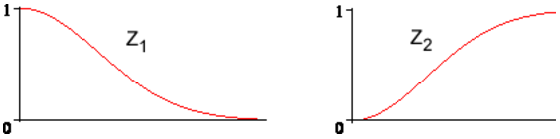
\includegraphics[scale=0.9]{MappingFunctions.png}
\caption{membership functions}
\end{figure}

\textbf{Negation} is defined as $1-z$.  As a consequence of this, for any concept, $z = 0$ means the \textit{antithesis} of that concept.  For example $Z(young) = 0$ would mean �old�. Another consequence is that the point at $z = 0.5$ is the \textit{point of neutrality}, which is where a concept is neither true nor false.

Some concepts (such as ``chair'', ``absurd'') do not have natural opposites.  For these concepts, $z = 0$ means the \textit{complete absence} of the qualities in question.

%Naturally opposite concepts can be represented by 2 predicates, $Q^+$ and $Q^-$, with $z$ values joined at 0 in the middle:
%\begin{table}[H]
%\hspace*{4cm} 
%\begin{tabular}{c c c}
%{\bfseries $z^+ = 1$} & {\bfseries $z^+ = z^- = 0$} & {\bfseries $z^- = 1$}\\
%\multicolumn{3}{c}{$|$\textemdash\textemdash\textemdash\textemdash\textemdash\textemdash\textemdash+\textemdash\textemdash\textemdash\textemdash\textemdash\textemdash\textemdash$|$}\\
%hot       & room temperature & cold\\
%masculine & unisex           & feminine\\
%pretty    & average looks    & ugly\\
%young     & middle age       & old
%\end{tabular}
%\end{table}

Negation can cause some confusion because ``not young'' can mean either ``middle age'' or ``old''.  The only treatment of fuzzy negation that is entirely consistent with our common-sense is to distribute probabilities over fuzziness,  which will be developed after \S\ref{sec:P(Z)-defined}.

The interpretation of the parameter $\xi$ in eqn (\ref{eqn:Z-squashing-fns}) is that it marks the \textit{point of neutrality} on the x-axis, for which z=0.5.  This is illustrated as follows:  we map the human age $x$ to the $\catZ$-concept of ``young'', where I (subjectively) define ``40 years old'' as the neutral point of ``young'':
\begin{figure}[H]
\centering
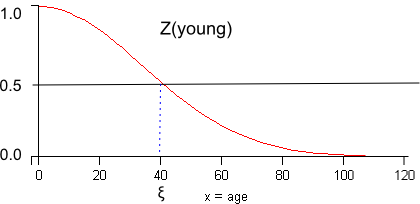
\includegraphics{neutral-point.png}
\caption{neutral point}
\end{figure}
This means, after 40, one gets more and more ``not young'' according to this definition.  

Thus the numerical scale of $\catZ$ is:\\
\begin{table}[H]
\parbox{3cm}{\caption{}}
\begin{tabular}{|l||l|}
\hline
{\bfseries z} & {\bfseries interpretation}\\ \hline
1.0     & definitely or extremely\\
0.9     & very\\
0.7-0.8 & moderately\\
0.6     & slightly\\ \hline
0.5     & neutral\\ \hline
0.4     & slightly not\\
0.3-0.2 & moderately not\\
0.1     & very not\\
0.0     & definitely not\\ \hline
\end{tabular}
\end{table}

Note:  A question has been raised whether we can define opposite concepts with 2 predicates, $Q^+$ and $Q^-$, with $z^+$ and $z^-$ joining at 0 in the middle.  This is not entirely satisfactory because the negation of $Q^+$ would not \textit{cover} $Q^-$, nor vice versa.  Therefore, the choice of $z=0.5$ as neutrality point is quite essential.

\section{Why Z obeys min-max calculus}
\label{sec:min-max-VS-sum-product}

Probabilities obey sum-product calculus;  $\catZ$ obeys \textbf{min-max calculus} \citep*{Zadeh1965}, ie:
\begin{eqnarray}
z_1 \Zand z_2    & \defeq &  min(z_1, z_2) \\
z_1 \Zor   z_2    & \defeq &  max(z_1, z_2).
\end{eqnarray}
My justification for min-max is as follows:

As an example, consider the statement:\\
\hspace*{1cm} S1: \textit{``John have had sex with 1000 women''}\\
but it turns out that all those women had only had cybersex with him.  Most people would agree that cybersex is not quite the same as real sex (some may say it's a borderline case ($z=0.5$)).  Suppose we subjectively think that cybersex is 0.7 real sex (as a measure of degree), then what would be the ``degree of truthfulness'' of the statement S1 (assuming that we accept the fact that he had cybersex with 1000 women)?

If we use the sum-product calculus (as with probabilities), the answer would be $ 0.7^{1000} $ which is almost zero.

Whereas if we use the min-max calculus, the answer would be $min\{0.7, 0.7, ...\} = 0.7$.  So, did John have sex with 1000 women?\\
\hspace*{1cm} answer A:  ``Of course not.''\\
\hspace*{1cm} answer B:  ``Well... sort of.''\\
My view is that the conjunction of 1000 vague events should have the same vagueness as the individual events.  You may try this with other examples of graded events.

%If this is still unclear, consider more examples:\\
%\hspace*{1cm} S2: ``John ate 100 hotdogs in 1 hour'' (but they are all mini-hotdogs)\\
%\hspace*{1cm} S3: ``John defeated 20 chessmasters'' (but they each offered him 2 free moves)\\
%\hspace*{1cm} S4: ``John is fluent in 20 languages'' (but they are computer programming languages)\\
%\hspace*{1cm} S5: ``John finished reading 50 novels'' (but they are all abridged versions)\\
%Would you accept these statements as \textit{partially} true?  Min-max calculus would grant that they are ``somewhat'' true.  Sum-product, however, would infer that they are effectively completely false.

\section{Axiomatic description}
\label{sec:fuzziness-axioms}

In summary, $\catZ$ is the relaxation of the classical-logic view that a statement is either true or false;  {true, false} is relaxed to [0,1].

Here is a set of axioms that describes $\catZ$:

Z1. $z \in [0,1]$ \\
Z2. $z$ varies continuously within $(0,1)$ \\
Z3. $z=0.5$ is the point of neutrality\\
Z4. $\catZ$ obeys min-max calculus when applied by logic conjunction and disjunction

The meaning of Z2 is yet to be clarified.  For now I'd just state it informally.  Also, it would be nice to formulate $\catZ$ calculus in a way similar to Cox's postulates for probabilities, but that is not my current priority.

\section{A fuzzy paradox}

A common problem in fuzzy logic is concerning the truth value of statements such as ``Q and not Q''.  It can be resolved using our understanding of $\catZ$ negation:

Suppose $Z(tall(john)) = 0.6$ (which means that John is slightly tall)\\
then\\
\hspace*{1cm} $ tall(john) \Zand \neg tall(john) = 0.4$ (which means this is slightly false)\\
\hspace*{1cm} $ tall(john) \Zor \neg tall(john) = 0.6$ (which means this is slightly true)

On the other hand, if $Z(tall(john)) = 0.4$ (which means that John is slightly short)\\
then\\
\hspace*{1cm} $ tall(john) \Zand \neg tall(john) = 0.4$ (which means this is slightly false)\\
\hspace*{1cm} $ tall(john) \Zor \neg tall(john) = 0.6$ (which means this is slightly true)

All these are reasonable conclusions.

\section{Unifying AND and OR}
\label{sec:unifying-AND-and-OR}

We seek to unify AND and OR by using a single operator $\varodot$ with a parameter $\theta$ such that when $\theta = 0$ it reduces to AND and when $\theta = 1$ it becomes OR.

A simple way to define $\varodot$ is:
\begin{equation}
X_1 \bigodot_\theta X_2 = (1-\theta) (X_1 \Zand X_2) + \theta (X_1 \Zor X_2).
\end{equation}

This animation shows the graph of $X_1 \varodot X_2$ as $\theta$ varies (requires Adobe Reader to trust this document):

\begin{figure}[H] %[ht]
\includemovie[
  poster,
  text={\small(** Click to play **)}
]{354px}{523px}
{unified-AND-OR.swf}
\end{figure}

\section{``Soft'' min-max and concept learning}

\{ TO-DO:  I have some doubts about this section; the argument is a bit unclear.  Maybe soft min-max are unnecessary afterall... \}

As an example, these are 2 exemplars of ``chair'' that most people consider to be typical:
\begin{figure}[H]
\centering

\includegraphics{2-chairs.png}
\end{figure}
Usually, the old-fashioned chair is 4-legged and is made of wood; and the office swivel chair can rotate and has wheels.  These are the \textbf{sfeatures} of the exemplars stored in memory.  It would be atypical for a wooden chair to have wheels and have a seat that can rotate above the 4 legs.  So, even though both chairs are very typical chairs, their features cannot be exchanged freely while maintaining the same level of typicality.

\hspace*{1cm} \begin{tabular}{|l|l|l|} \hline
\textbf{features}            & \textbf{degree} &\\ \hline
wooden $\Zand$ 4-legged     & 1.0             & typical old-fashioned chair\\
rotating $\Zand$ has wheels & 1.0             & typical office chair\\
has wheels $\Zand$ 4-legged & 0.9             & atypical chair\\
\hline
\end{tabular}

It seems that crisp min and max cannot represent this (but I may be mistaken about this point).  Anyway, I created a ``soft'' version of min-max (the idea is to use $z_1, z_2$ as their own weights in a weighted average):

\hspace*{1cm} \begin{tabular}{|l|l|}
\hline
{\textbf{soft min (= AND)}} & {\textbf{soft max (= OR)}}\\ \hline
\rule[-7mm]{0mm}{16mm} 
$\displaystyle z_1 \; \widetilde{\wedge} \; z_2 = \frac{z_1 (1-z_1) + z_2 (1-z_2)}{1 - z_1 + 1 - z_2} $
& $\displaystyle z_1 \; \widetilde{\vee} \; z_2 = \frac{z_1 z_1 + z_2 z_2}{z_1 + z_2} $ \\
\hline
\end{tabular}
\parbox{4cm}{\begin{equation}
\label{eqn:soft-min-max}
\end{equation}}

It can be verified that soft- min and max satisfy the boundary conditions of classical logic, provided that we make $0/0 = 1$ in the min case.

\begin{figure}[H]
\centering
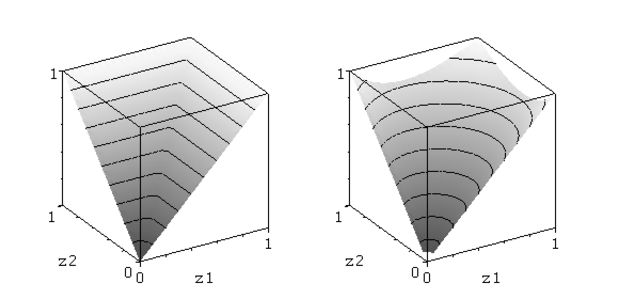
\includegraphics[scale=0.9]{soft-max.png}
\caption{comparison of max and soft max}
\end{figure}

\section{$\catZ$ modifiers}
\label{sec:Z-modifiers}

To make $\catZ$ logic more versatile, we need to augment it with \textbf{modifiers} which correspond to natural-language hedges like:\\
\hspace*{1cm} extremely \hspace*{1cm} very \hspace*{1cm} moderately \hspace*{1cm} slightly\\
so we can express things like:\\
\hspace*{1cm} $\mbox{lukewarm} \leftarrow \mbox{moderately(warm)}$\\
\hspace*{1cm} $\mbox{obese} \leftarrow \mbox{very(fat)}$

In general, we can define a $\catZ$-modifier as a function $\Gamma: [0,1] \rightarrow [0,1]$,
\begin{equation}
z_0 := \Gamma(z_1)
\end{equation}
We further restrict the class of $\Gamma$ to make the system simpler.  I suggest to use Gaussian functions with the mean $z^*$ as a parameter, and the variance would be fixed to a certain constant.  So
\begin{equation}
z_0 := \Gamma(z_1; z^*) = \frac{1}{\sigma \sqrt{2 \pi}} e^{- (z_1-z^*)^2 / 2 \sigma^2}
\label{eqn:fuzzy-moderator-Gaussian}
\end{equation}
For example, the $\Gamma$'s for ``slightly'' and ``very'' can be:
\begin{figure}[H]
\centering
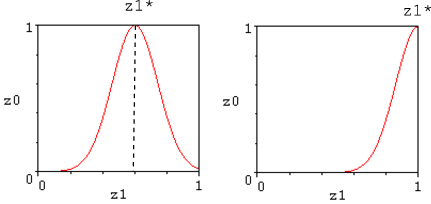
\includegraphics[scale=0.9]{fuzzy-modifiers.png}
\caption{Fuzzy modifiers with $z^* = 0.6, 1.0$}
\end{figure}

We can have better control over the shapes of $\Gamma$ by using other functions and having more parameters, but I suspect that such sophistication is not needed for common-sense reasoning.

For example, we can define ``lukewarm'' as ``warm'' with $z \in [0.6,0.8]$, or:\\
\hspace*{1cm} $\mbox{lukewarm} \leftarrow \Gamma_{0.6}(\mbox{warm}) \Zand \Gamma_{0.8}(\mbox{warm})$\\
using 2 $Gamma$'s with fixed variances.  The result is the blue curve on the left.  We get the interval [0.6,0.8] by taking $> 0.5$ as true, and thus ``lukewarm'' would be a binary predicate.
\begin{figure}[H]
\centering
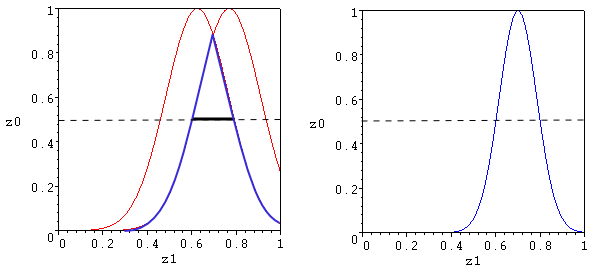
\includegraphics[scale=0.9]{Gamma-for-lukewarm.png}
\caption{Two representations of ``lukewarm''}
\end{figure}
On the other hand, if we use a tailored $\Gamma$ to represent ``lukewarm'' on the right, it would be a $\catZ$-predicate with continuous values like ``slightly lukewarm'' and ``very lukewarm''.  This seems to be unnecessarily sophisticated.

\{ TO-DO:  One problem with this method is that the predicate ``lukewarm'' changes abruptly at the boundaries.  Another example is ``middle-aged''.  \}

\{ TO-DO:  Prove that combinations of $\Gamma$ and $\Zand ,\; \Zor$ can be universal approximators. \}

\section{$\catZ$-conditionals}
\label{sec:Z-conditionals}

In general, inference is driven by rules.  In $\catZ$ logic all rules take the form of $\catZ$-conditionals.  A $\catZ$-conditional is specified by a combination of min's and max's (similar to DNFs (disjunctive normal forms) in classical logic):
\begin{equation}
z_0 \; := \; \bigZor_i \; \bigZand_j \; \Gamma(z_{ij})
%z_0 \; := \; \widetilde{\bigvee_i} \; \widetilde{\bigwedge_j} \; \Gamma(z_{ij}; z^*_{ij}, v_{ij}) \, = \; \widetilde{\bigvee} \; \{ z_{11} \, \widetilde{\wedge} \, z_{12} \, \widetilde{\wedge} \cdots, z_{21} \, \widetilde{\wedge} \, z_{22} \, \widetilde{\wedge} \cdots, \, \cdots \}
\end{equation}

Notice that a $\catZ$ rule directly assigns a $\catZ$ value to $z_0$ \textit{without the use of an implication operator}, which is very different from traditional fuzzy logics:

\subsection{Traditional fuzzy logic}

A fuzzy implication is a map $\Rightarrow: [0,1] \times [0,1] \rightarrow [0,1]$ satisfying these boundary conditions from binary logic:\\
\hspace*{1cm} \begin{tabular}{|l|l|l|} \hline
$\Rightarrow$ & 0 & 1\\ \hline
0             & 1 & 1\\
1             & 0 & 1\\ \hline
\end{tabular}

A fuzzy implication statement:  $(Z_1 \Zand Z_2) \Rightarrow Z_0$  means that the fuzzy values $z_0,z_1,z_2$ obey the equation:
$$ ((z_1 \Zand z_2) \Rightarrow z_0) = z_c $$
where $z_c$ is the truth value of the implication statement.  Compared to my approach, this has an extra level of indirectness.  Is it really necessary that we know the truth value of an implication statement?  (Cf \S\ref{sec:P-and-ClassicalLogic}: In probabilistic logic, the probability conditional $P(A|B)$ serves as the implication statement, but we usually do not ask about its own probability.)  One trouble with traditional fuzzy logic is that we cannot even perform \textit{modus ponens} unless we allow interval fuzzy values.\footnote{Suppose we define the operators for a very simple fuzzy logic: $a \Rightarrow b \equiv \neg a \vee b$, $\neg a \equiv 1-a $, and $a \vee b \equiv min(a,b)$.  \citep*{Kenevan1992} has given an inference algorithm for this logic, but it is very complicated and involves interval fuzzy values, and so is not very suitable for further complex development.}

% Now given that $Z_1 = z_1$ and $Z_1 \Rightarrow Z_0$, ie $ (z_1 \Rightarrow z_0) = z_c $, ie $min(1-z_1,z_0)=z_c$ we still cannot determine $z_0$.}

% TO-DO:  weighted soft min-max may not be needed, if we have fuzzy modifiers

%An example involving vagueness: ``smart''\\
%\hspace*{1cm} smart $\leftarrow$ humorous\\
%\hspace*{1cm} smart $\leftarrow$ articulate\\
%\hspace*{1cm} smart $\leftarrow$ blah

\section{Combining $\catB$, $\catP$, $\catZ$}
\label{sec:combinePZ}

\subsection{The truth value P(Z)}
\label{sec:P(Z)-defined}

How to combine $\mathcal{P}$ and $\catZ$?  The answer is simple because there is no other choice:  the semantics of probabilities dictate that $\mathcal{P}$ must be \textit{distributed over events}.  In the current system, events are either $\mathcal{B}$ or $\catZ$ (the latter are \textit{continuous} events).  So we \emph{distribute $\mathcal{P}$ over $\mathcal{B}$ and $\catZ$}.  In this sense, fuzziness is more fundamental than probabilities.

If a $\catZ$ value is uncertain --- for example, we may not be sure how tall Mary is (the $\catZ$-value of her tallness may be 0.6-0.8, say, so we can assume a uniform probability distribution over the interval [0.6,0.8] which is the green rectangle below) --- and we can approximate it by a Beta distribution over $\catZ$ with a mean at 0.7 and the same variance:
\begin{figure}[H]
\centering
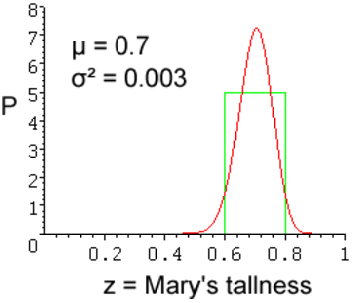
\includegraphics[scale=0.9]{P-over-Z-Marys-Tallness2.png}
\caption{an example $\mathcal{P}(\catZ)$ distribution}
\end{figure}
where the probability density should sum to 1: $ \int^1_0 P(z) dz = 1 $.

On the other hand, if a $\mathcal{P}$ value is uncertain, we simply \textit{ignore} its error (eg, by choosing the mid-point of a P-interval).  \S\ref{sec:PointValued} tried to justify this.

The following commutative diagram shows the relationship between $\mathcal{B}$, $\mathcal{P(B)}$, $\catZ$, and $\mathcal{P(Z)}$:

\begin{figure}[H]
\centering
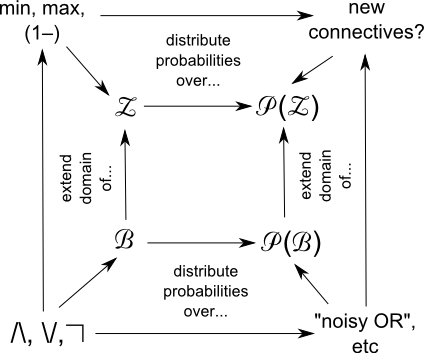
\includegraphics[scale=0.8]{P(Z)-commutative-diagram.png}
\end{figure}

The inner square contains the 4 types of truth values.  The outer square are the corresponding logics, showing their logical operators.  The radial arrows point to the ``underlying sets'' of TVs.

\subsection{An example}

Consider the common sense notion:\\
\hspace*{1cm} \textit{The richer a person, the more powerful s/he is.}\\
Note that this rule is inexact:  there are exceptions (where some rich people are not powerful and some powerful people are not rich) and deviations (the data points do not fall on a straight line):

\begin{figure}[H]
\centering
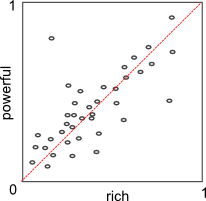
\includegraphics{rich-vs-powerful.png}
\end{figure}

There are reasons to believe that the identity function (red line) represents the least-error regression function:  first, the $\catZ$ values are in ``natural scale'' (ie, $z=1$ corresponds to $\infty$) so $(z_1,z_2)$ at $(1,1)$ is obvious if we accept the original statement;  secondly, when $z_1 = 0.5$, the person is neither rich nor poor, and we should have nothing to say whether the person is powerful or not, as far as the original statement is concerned.

\underconst

\subsection{Unifying all truth values to $\catPZ$}
\label{sec:unifying-P(Z)}

Up to now there are 4 possible TV types:
\begin{table}[H]
\parbox{3cm}{\caption{}}
\begin{tabular}{|l|l|l|} \hline
\multicolumn{3}{|c|}{\textbf{truth values}}\\ \hline
category                   & meaning                                      & definition \\ \hline
$\mathcal{B}$              & binary                                       & $b \in \{true, false\} $\\
$\catZ$              & fuzzy                                        & $z \in [0,1] $\\
$\mathcal{P}(\mathcal{B})$ & $\mathcal{P}$ distributed over $\catZ$ & $ P(b=false) = p_0 $\\
                           &                                              & $ P(b=true) = p_1 $\\
$\mathcal{P}(\catZ)$ & $\mathcal{P}$ distributed over $\catZ$ & $ P(z=z_1) \sim Beta(z_1) $\\ \hline
\end{tabular}
\end{table}
I find that they can be unified to type $\mathcal{P(Z)}$, which can make things simpler.  Below is how to represent the other 3 TV types as $\mathcal{P(Z)}$:

\subsubsection{Type $\mathcal{B}$}

Some variables have a strong ``binary flavor''.  For example, in common sense, a person is either dead or alive, although a more nuanced view will have grades of being dead.  If deadness is a $\catZ$ variable, z = 0 would be ``definitely alive'', z = 1 would be ``definitely dead'' (eg reduced to ash), and z = 0.5 would correspond to a state that is difficult to classify as dead or alive, eg a brain-dead, vegetative state.  z = 0.7 may be a state that is more dead than brain-dead and yet more alive than ash, eg --- I have to pause for a while to think of an example --- a body under cryonic preservation.  And z = 0.4 may be some kind of near-death experience.  Anyway, one can expect the probability distribution of $z_{dead}$ to be polarized with a trough in the middle.  This can be represented by a Beta distribution with a large variance:
\begin{figure}[H]
\centering
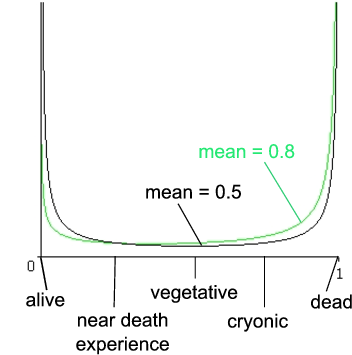
\includegraphics{deadness.png}
%\caption{Z = deadness}
\end{figure}
When the polarization gets extreme (eg the toss of a coin is either head or tail), the distribution becomes a $\bigsqcup$ shape.  The degree of polarization (ie amount of variance) can be estimated statistically, if data is available.

It appears that all common-sensical $\mathcal{B}$ variables are actually \textbf{polarized} $\catZ$ variables.  Another example is a person being either married or not married, and there are grey areas like gay marriage or marriage for the green card, etc.

Actually the Beta distribution (eqn \ref{eqn:beta-distro}) is capable of representing 3 types of characteristics (with $a = 1$ and $b = 1$ as points of transition separating the 3 regimes):
\begin{figure}[H]
\centering
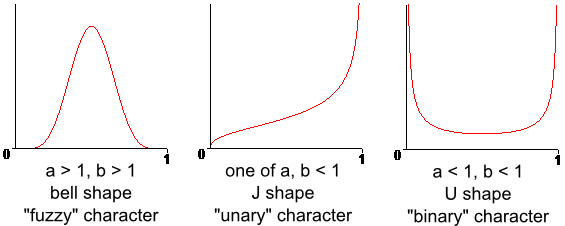
\includegraphics[scale=0.8]{binary-fuzzy-unary-characters.png}
\end{figure}
The unary type represents concepts such as ``normal'', ``broken'', ``healthy'', or ``natural''.  In such concepts, the state at $z = 1$ can be clearly defined (eg, John was perfectly healthy when he was a kid), but as we approach $z = 0$ the cases become very improbable and inexhaustible (eg, it is impossible to find a person who is ``utmost unhealthy'' because it is always possible to think of more extreme and improbable unhealthy ways.  Also, committing suicide is not the limiting case --- suicide is not the same as unhealthy --- so the interval is open-ended.)

\textbf{About the mean and variance.}  In the fuzzy regime, the smaller the variance, the shaper the peak and thus the more confident we are about the $\catZ$ value;  The variance is a measure of confidence in this regime.  In the binary regime, the greater the variance, the more \textit{polarized} the distribution becomes;  The variance is a measure of binary character.  In the unary regime, the meaning of the variance is unclear.

%The transition occurs at $a = 1$ or $b = 1$:
%\begin{figure}[H]
%\centering
%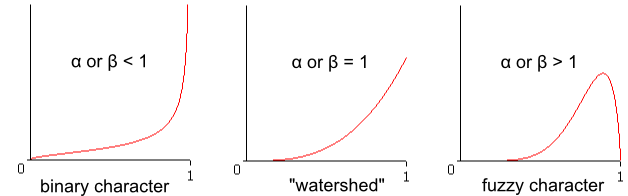
\includegraphics{Beta-distro-watershed.png}
%\end{figure}

%If we know the mean $\mu$, the variance at the transition point is given by:
%\begin{equation}
%v_0 = \frac{(\mu-1)^2 \mu}{2-\mu} \quad or \quad v_1 = \frac{\mu^2(1-\mu)}{\mu+1}
%\end{equation}
%The important thing to understand is that the meaning of the variance is \textit{reversed} after the transition point.  Usually, the variance increases when the sharpness decreases.  But when we have ``binary character'', the distribution gets sharper when variance \textit{increases}, as the probability mass is being pushed to the extremes.  Thus, greater variance here means greater precision.

%Something is wrong here.  There is not one transition point, but a band?  The transition occurs when, giving more variance will give more to the poles.  But this is always true!  So there is no clear cut boundary.  At one extreme is variance = 0, where one of $a, b = \infty$, or when one of $a, b = 0$.  When the variance gets to its maximum, $a = b = 0$ and we have fractional Dirac deltas at the poles, which is fine with the binary interpretation.  The question is when does the binary regime start?  It seems that there is really a transitional band.  It is difficult to say that the J shape is binary or fuzzy.  Examples of J are ``normal'', ``sane'', ``healthy'', ``natural'', etc.  J may be called the ``unary'' regime.

%\textbf{About the mean.}  In the fuzzy regime, the mean is at or near the most probable value, and the variance is a measure of uncertainty about the mean.  In the binary regime, the interpretation is different.  Here, the most probable values are at 0 or 1, and the mean indicates which extreme has higher probability.  The variance indicates the degree of polarization --- the higher, the more ``binary''.

To illustrate this with an example:  In the fuzzy regime, I can say ``John is 0.7 dead because he's in a cryonic state'', and I can use a small variance to indicate that I am confidence that John is in a cryonic state and \textit{not elsewhere}.  In the binary regime, however, I can only indicate the probability of ``John being dead or not'' where ``dead'' is an ``either-or'' condition.  The highest probabilities are concentrated at 1 (``definitely dead'') and 0 (``definitely alive''), and the cryonic state has low probability.  Under this regime there is no way to accentuate (make more probable) the cryonic state --- one can only do so in the fuzzy regime.  This is exactly what we would expect with a binary variable.

%This has consequences when we perform belief revision (\S\ref{ch:belief-revision}), when we need to update variances.

%Once we established that a variable is polarized, what if we then assert its probability?  Eg P(dead) = 0.7?  This is interesting.  Equally interesting, is when we know P(dead) = 0.7, and then assert its polarity.

\subsubsection{Type $\catZ$}

We can create a $\mathcal{P(Z)}$ distribution with a peak around $z$.  The variance depends on how confident we are of the $z$ value.  If unspecified, we can assign a typical variance to it.

\subsubsection{Type $\catPB$}

For example, ``Mary is probably married'', with p = 0.8.\\
ie \hspace*{1cm} $P(married) = 0.8, \quad \quad P(\neg married) = 0.2$.\\

In general, for any $\mathcal{P(Z)}$ variable $Z$, especially in the binary regime, one can set the probability of ``Z'' (viewed as a binary event) to be equal to the probability mass for $z \geq \frac{1}{2}$ which is given by the CDF of the Beta distribution, ie, the regularized incomplete Beta function:
$$ F(x; a, b) = \frac{ B(x; a, b) }{ B(a, b) } = I_x(x; a, b) $$
where $B(x)$ is the incomplete Beta function:
$$ B(x; a, b) = \int^x_0 t^{a-1} (1-t)^{b-1} dt \mbox{.}$$
Thus
$$ P(Z = \mbox{true}) = P(z \ge \frac{1}{2}) = 1 - P(\Zneg Z) = 1 - P(z < \frac{1}{2}) = 1 - I_x(1/2; a, b) $$

The desired mean $\mu$ can be solved from:
\begin{eqnarray}
I_x(1/2; a, b) = p\\
\mu = a/(a+b)
\label{eqn:mean-and-p}
\end{eqnarray}

An interesting observation:  As the variance $v$ increases, it eventually reaches a maximum $v_{max}$ where $a=b=0$ and the Beta distribution is undefined.  From Mathematica experiments, if we keep $ \mu = a / (a+b) $  fixed:\\
$$ \lim_{a,b \rightarrow 0} I_x(1/2) = \mu - 1 $$
This implies that, in the extreme polarized case:\\
$$ p = 1 - I_x(1/2) = 1 - (1 - \mu) = \mu $$

%The mean is related to $p$ by the simple formula (I'm assuming that the real distribution is like the rectangular distribution and therefore I find it's mean):
%
%\mu = \begin{cases}
%1 - \frac{1}{4p} & \quad 1 \geq p \geq \frac{1}{2} \\
%\frac{1}{4(1-p)} & \quad \frac{1}{2} > p \geq 0
%\end{cases}
%\label{eqn:mean-and-p}
%\end{equation}

The variance represents the degree of polarization of the variable, which varies from one variable to another, and can be quite arbitrary if unspecified.

%The inverse of eqn (\ref{eqn:mean-and-p}) is (with an extension to cover extremes):
%\begin{equation}
%p = \begin{cases}
%1                  & \quad \mu > 0.75 \\
%\frac{1}{4(1-\mu)} & \quad 0.75 \geq \mu \geq 0.5 \\
%1 - \frac{1}{4\mu} & \quad 0.5 > \mu \geq 0.25 \\
%0                  & \quad 0.25 > \mu
%\end{cases}
%\label{eqn:mean-to-p-conversion}
%\end{equation}

Inference of $\mathcal{P(Z)}$ logic will be treated in \S\ref{ch:inference}.

%\section{PZ logic formulated as FOL axioms}
%
%In this section I give the complete axioms for PZB logic, expressed in FOL.  That means, a FOL system will have the power of PZB logic when equipped with these axioms.  Thus, this allows us to build an AGI using a FOL inference engine as the core.

%ref1:  truth-value(s1, mean1, variance1)
%ref0:  truth-value(s0, mean0, variance0)
%
%1. How to represent a rule?  eg  bachelor :- male & ~married
%rule-and(bachelor, male, not_married).
%rule-not(not_married, married).
%
%2. How to deduce the TV of s0 given s1?
%retract(ref0).
%truth-value(s0, new-mean, new-variance).

%\section{Outstanding problems}

%1. There will be many factors.  It seems that the structural organization of factors is more important than numerical curve fits.

%2. Often I feel that the numerical values aren't that important at all.  Also I feel that there are many rules that are just B -- for example, $smart \leftarrow creative$.  Even if we have a Z rule, we should be able to talk about the B counterpart.  This is very perplexing... the Z rule may take away the meta-reasoning ability of B rules...?  But the B rule will retain that ability.  Maybe the Z rule can also have the ability of meta-reasoning?  That 'creative' is a component of 'smart'?

%3. The exact form of $P(Z)$ can be irregular, especially when it is given by several factors.

%4. ``Almost P (interpreted as binary)'' is ``close to P (interpreted as Z) $\wedge$ not P (interpreted as binary)''.  So it can be a strictly-B rule with a Z-literal translated to B.  But if the Z-literal is ``not that close to P'' then ``almost P'' may be partially true.  ``Almost P'' can be slightly true, slightly not true, very true etc.  And that seems to depend on the evaluation of ``close to P''.  Because ``close to P'' can be Z, then it seems that ``almost P'' can be Z too.  

%5. The question is whether ``almost P'' is B or Z.  Maybe in various contexts it can be both?  Or may be if it is ``very almost'' then we can as well make it B.  But if it is ``slightly not almost'' then we should make it Z.

%6. The problem now seems to be that we need meta-level intervention to decide what kind of TVs to use.  But the base logic (object-level logic) has difficulty deciding on its own.  This is a problem because the base logic is not well-defined.  We need some simple rules to decide what kind of TVs to use.

%7. It's obvious we need a choice of TVs.  In the ``almost'' case... there is perhaps a distinction between base logic and meta-logic, but this distinction is orthogonal to the choice of TVs.  Maybe there is always a choice of TVs but it is too sophisticated for the base logic?  But somehow the base logic has to make a choice... 

%8. Do rules have ``intrinsic'' TVs for each slot?

%9. Another problem is how to learn B rules *gradually*?  Perhaps we start with P(B) rules and then their P's tend to $\{0,1\}$?  How about Z rules -- do they ever turn into B rules?  Maybe some of the predicates turn binary?
